\documentclass[11pt]{article}
\usepackage{amsmath, amssymb, hyperref}
\usepackage{amsthm}
\usepackage{geometry}
\usepackage{graphicx}
\usepackage[backend=biber]{biblatex}
\addbibresource{../references.bib}
\newtheorem{lemma}{Lemma}
\newtheorem{definition}{Definition}
\newtheorem{remark}{Remark}
\geometry{margin=1in}
\title{\LARGE The Abstract Universe Project}
\author{Juha Meskanen}
\date{2019 -- \today}

\begin{document}

\maketitle

\section{Introduction}

In this framework, we reject the presumption that spacetime or particles are ontologically fundamental \cite{wheeler1990it} \citation{zuse1970calculating}. We show that the universe is made of abstract information, provided only four observable assumptions hold. The assumptions are observationally grounded regularities evident in both physics and computation. These assumptions are minimal, falsifiable, and intentionally free of ontological commitments. From them, we derive a conclusion: the universe must be fundamentally informational, and all informational states that satisfy these assumptions already exist.

The framework developed assumes no primitive physical substrate—no predefined spacetime, particles, or fields. Everything we observe, from matter to consciousness, is modeled as an emergent structure within a fundamentally informational universe.


\section*{The Observer Prevalence Principle}

Let $n$ be a fixed number of bits. Let $\mathcal{U}_n = \{0,1\}^n$ denote the set of all $2^n$ binary strings, interpreted as candidate universes. Let $\mathcal{O}_n = \{0,1\}^n$ denote the same set, interpreted as candidate observers.

Define a \textbf{compatibility function}
\[
      \mathrm{Compat}: \mathcal{O}_n \times \mathcal{U}_n \rightarrow \{0,1\}
\]
such that $\mathrm{Compat}(o, u) = 1$ if observer $o$ can exist within universe $u$ under a chosen observer model (e.g., memory encoding, trajectory embedding, structural motif match), and 0 otherwise.

\begin{definition}[Observer Prevalence Principle]
      The \emph{subjective probability} that a given observer $o \in \mathcal{O}_n$ experiences a particular universe $u \in \mathcal{U}_n$ is proportional to the number of universes compatible with $o$:
      \[
            \Pr(u \mid o) \propto \mathrm{Compat}(o, u).
      \]
      Equivalently, the most probable universe an observer experiences is the one maximizing the number of observer-compatible instances:
      \[
            u^* = \arg\max_{u \in \mathcal{U}_n} \sum_{o \in \mathcal{O}_n} \mathrm{Compat}(o, u).
      \]
\end{definition}

This principle implies that the observed universe is biased toward configurations that support the maximal number of observers isomorphic to the subject, leading to emergent regularities (e.g., smooth physical laws, coherent time evolution) that favor observer persistence.

\begin{remark}
      The special case where an observer $o$ is identical to a universe $u$ (i.e., $o = u$ and $\mathrm{Compat}(o, u) = 1$ trivially) defines a fixed point of maximal internal consistency. This limiting case represents an informational singularity—an observer-universe with no internal entropy or external reference.
\end{remark}



\section*{A Technical Introduction to an Observer-Centric, Information-Theoretic Theory of Everything}

This theory proposes that \textbf{physical reality emerges from pure information}, with no need to assume pre-existing spacetime, particles, or energy. At the center is the following hypothesis:

\begin{quote}
      \textit{The most probable universe is the one that minimizes the informational description of the observer.}
\end{quote}

The universe is modeled as a set of finite-length bitstrings evolving over discrete time steps. Observers are defined as memory-encoded patterns within those bitstrings. A universe is said to implement an observer if it contains a coherent embedding of the observer’s memory across time. Among all such universes, \textbf{those with minimal total description length} — i.e., those offering the best data compression of the observer — are statistically favored.

\subsection*{1. Observer-Centric Selection Principle}

The observer is not external to the universe but embedded within it. For a bitstring universe $U$, and an observer pattern $O$, we define the compatibility function $C(U, O)$ based on:

\begin{itemize}
      \item \textbf{Memory embedding}: The observer must find a consistent sequence of memory states in $U$.
      \item \textbf{Compression}: The joint configuration of $U$ and $O$ should have minimal Kolmogorov complexity.
\end{itemize}

Formally, we define the observer-weighted universe probability as:
\[
      P(U \mid O) \propto 2^{-K(U \mid O)}
\]
where $K(U \mid O)$ is the conditional Kolmogorov complexity of the universe given the observer. Universes with more regularity — i.e., more easily expressed using fewer bits — dominate the ensemble.

\subsection*{2. Wavefunction as Compression Algorithm}

A central insight of the theory is that the \textbf{wavefunction is not a physical field}, but a compression scheme — a compact encoding of possible observer-consistent universes. Sinusoidal patterns, being maximally compressible via Fourier bases, naturally dominate. This yields a statistical bias toward universes that exhibit \textbf{wave-like evolution}, which in turn gives rise to quantum interference, superposition, and smooth particle trajectories.

\subsection*{3. Time, Entropy, and the Observer's Horizon}

Time is modeled as an ordered super-set of bitstrings. Past states are constrained by observer memory; future states are undetermined but \textbf{filtered} through the compression mechanism (the wavefunction), yielding a \textbf{probabilistic projection} rather than deterministic evolution.

\begin{itemize}
      \item The \textbf{past} is the region of high similarity with observer memory.
      \item The \textbf{future} is a superposition of all possible continuations consistent with the observer’s wavefunction.
\end{itemize}

This leads to an asymmetric structure: \textbf{a classical past and a quantum mechanical future}, unified through entropy and informational symmetry.

\subsection*{4. Physical Laws as Emergent Regularities}

No physical constants are assumed. Instead, \textbf{laws of physics emerge as statistical biases} in the set of observer-compatible universes. For example:

\begin{itemize}
      \item \textbf{Particles}: Recurring spatial motifs across frames.
      \item \textbf{Fields}: Gradients in compressed observer-compatible configurations.
      \item \textbf{Gravity}: Emerges from local entropy gradients that attract compatible observer trajectories.
\end{itemize}

All such phenomena arise not from axioms of physics, but from the mathematics of information compression and observer self-location.

\subsection*{5. Simulation and Empirical Grounding}

A concrete implementation of this theory samples all possible spacetime bitstring paths of a given size and ranks them by wave-based compression with respect to an observer pattern. Visual plots (Section 6) confirm that high-scoring paths exhibit:

\begin{itemize}
      \item Increasing entropy over time (arrow of time)
      \item Emergent particle-like structures
      \item Smooth geodesic-like motion
      \item Quantum-like predictive uncertainty and interference
\end{itemize}

\section*{6. Quantum Mechanics as Emergent Compression Behavior}

To concretely demonstrate the emergence of quantum behavior, we simulate a simple setup: a fixed observer memory pattern embedded within a set of evolving bitstring universes of length $n=24$ over $T=12$ time steps.

\subsection*{Observer Encoding}

We define an observer pattern $O$ as a fixed 8-bit substring representing a memory trace (e.g., \texttt{11001010}). The simulation searches for universe histories $U$ in which this observer pattern recurs across frames with minimal change, favoring paths with:

\begin{itemize}
      \item High internal consistency (low entropy deviation)
      \item Compressibility under wave-like (Fourier) filters
\end{itemize}

\subsection*{Emergent Wave Patterns}

Figure~\ref{fig:observer-trace} shows a heatmap of bitstring space over time, where compatible paths exhibit constructive interference — producing sinusoidal probability densities resembling quantum mechanical wavefunctions.

\begin{figure}[h!]
      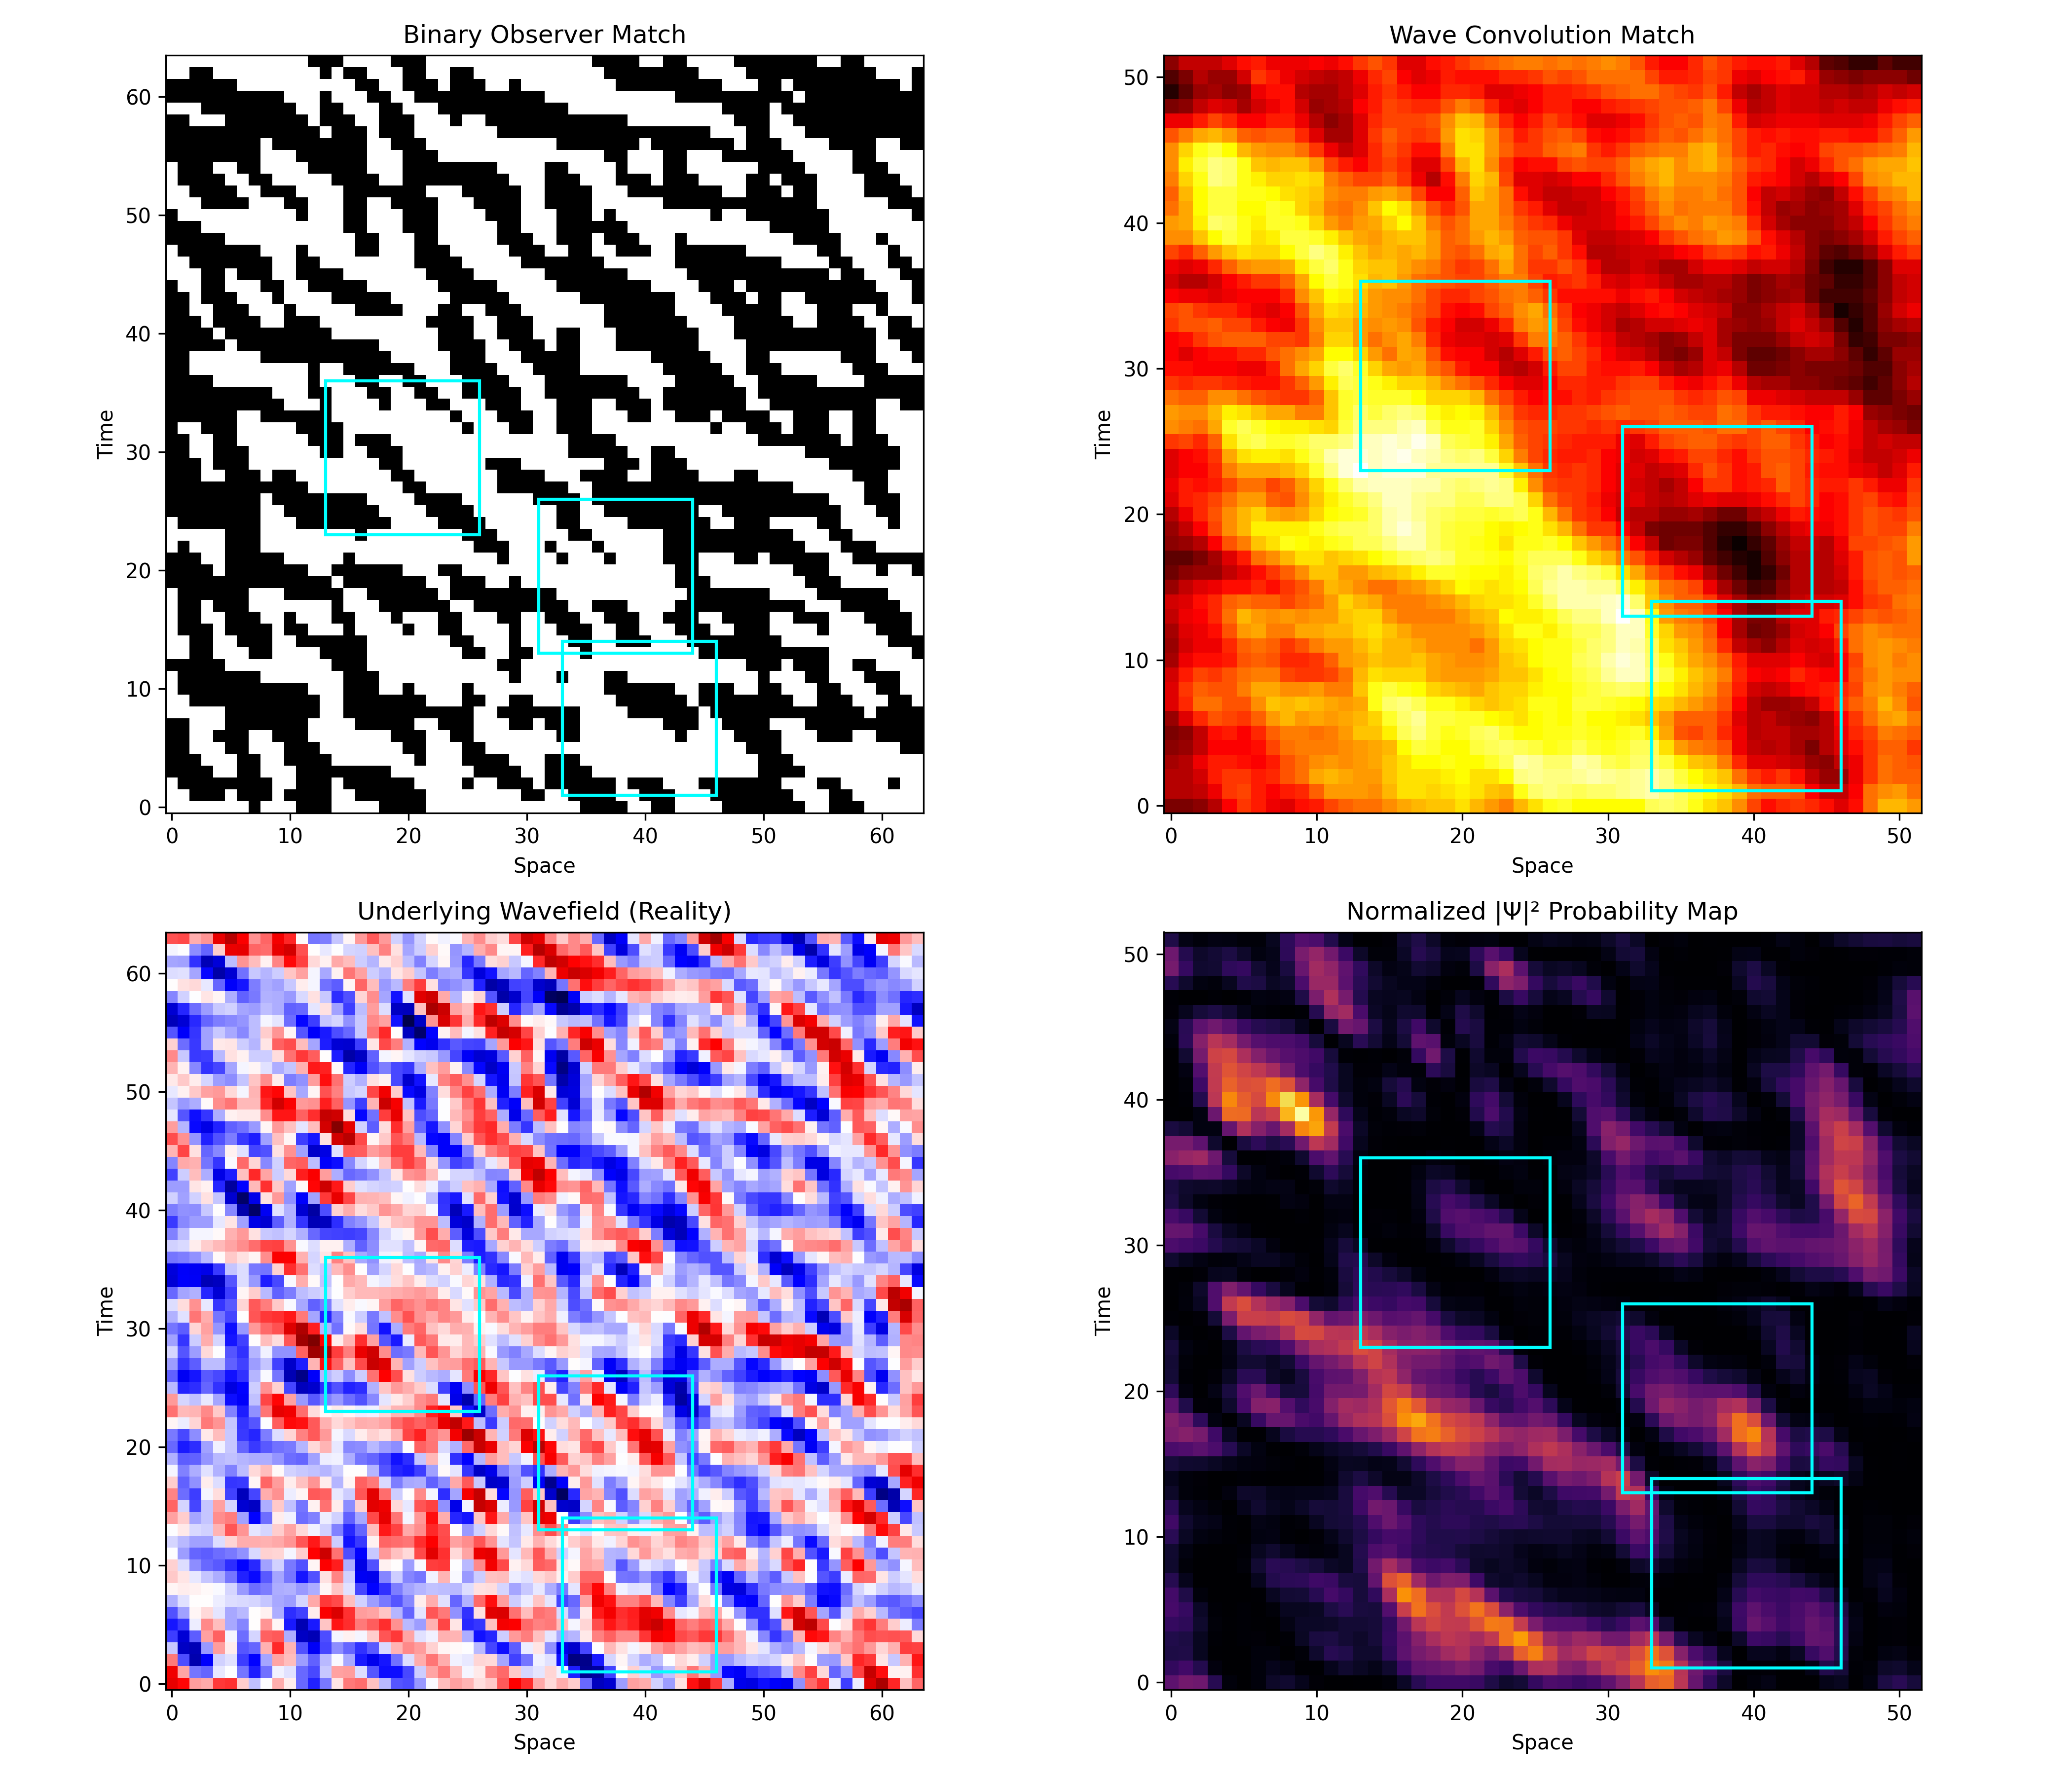
\includegraphics[width=1.0\textwidth]{figures/observer_wave_evolution.png}
      \caption{Heatmap of observer-compatible universe paths over 12 steps. High-similarity paths constructively interfere, producing wave-like amplitude envelopes.}
      \label{fig:observer-trace}
\end{figure}

\subsection*{Interference and Probability Amplitudes}

Due to bitstring superposition and compression bias, some paths amplify while others cancel — not unlike Feynman path integrals. This leads to:

\begin{itemize}
      \item Apparent interference patterns
      \item Probabilistic future branches weighted by compressibility
\end{itemize}

These results replicate familiar quantum behaviors from an entirely classical bit-based foundation.



\subsection*{Conclusion}

This theory redefines ontology: \textbf{reality is not made of matter but of compressible information}, with observers acting as statistical filters. The universe is not a singular entity but a probabilistic ensemble weighted by informational efficiency. And physics — all of it — is just the echo of a deeper algorithm: \textbf{find the wave that best describes you.}


\end{document}

